\documentclass[11pt,a4paper,twocolumn]{article}
\usepackage[utf8]{inputenc}
\usepackage[T1]{fontenc}
\usepackage{amsmath, amssymb, graphicx, booktabs, tikz}
\usepackage{microtype}
\usepackage[hyphens]{url}
\usetikzlibrary{arrows.meta, positioning, shapes.geometric}
\raggedbottom

\title{A graph-based framework for quantitative analysis of navigational complexity in indoor orienteering courses}
\author{}
\date{\today}

\begin{document}

\maketitle

\begin{abstract}
Indoor orienteering presents a navigational challenge distinct from
traditional forest orienteering: multi-floor venues, one-way passages, and
discontinuous map segments create a dense space of route choices within a
small physical area. This article introduces a graph-based framework for
modeling indoor venues and courses, defines a notion of route identity
based on visible stair crossings that makes exhaustive route enumeration
tractable, and describes a first difficulty scoring model calibrated
against published course-setting guidelines. The framework is implemented in
an open toolchain (web application, command-line tools, and analysis
libraries). We position this work as a foundation: the model, the enumeration
algorithms, and the collected data enable follow-up
research on difficulty scoring models, route-choice behavior, and course design.
\end{abstract}

\section{Introduction}

Indoor orienteering is a growing discipline in which competitors navigate
multi-floor buildings using specially drawn maps, typically with one map
segment per floor printed side by side. Compared to forest orienteering, the
navigational difficulty is concentrated in a small area: route choice is
dominated by \emph{which staircases to use} and constrained by one-way
passages, and the branching factor of decisions per minute is high.

Course setters today rely on qualitative difficulty guidelines, such as the
five-level color scale published by Stockholm Indoor
Cup~\cite{sic-difficulty}, and on personal experience. There is no established
quantitative method for assessing how difficult a leg or a course actually is,
nor for comparing difficulty across venues and events.

This article introduces a framework that makes such analysis possible. The
contributions are:

\begin{enumerate}
    \item a \textbf{graph model} of indoor venues that captures corridors,
          stairs, one-way constraints, and floor membership
          (Section~\ref{sec:model});
    \item a definition of \textbf{route identity} --- two paths are the same
          route if and only if they cross the same labeled stairs in the same
          order --- which reduces route enumeration from an intractable
          all-simple-paths problem to a tractable search over label sequences
          (Section~\ref{sec:routes});
    \item a first \textbf{difficulty scoring model},
          additive over stair crossings and branching points, mapped onto the
          established difficulty categories (Section~\ref{sec:scoring});
    \item an \textbf{open implementation} of the above, together with
          venue graphs, courses, and anonymized split-time data from real events for future validation
          (Section~\ref{sec:implementation}).
\end{enumerate}

We deliberately keep the scoring model simple and inspectable. The goal of
this first article is not a definitive difficulty measure, but a shared
vocabulary, data model, and algorithmic toolkit on which such measures can be
built and tested.

\section{Terminology}
\label{sec:terminology}

Indoor orienteering maps contain structural elements with no direct outdoor
counterpart. We use the following terms throughout.

\begin{itemize}
    \item \textbf{One-way passages:} areas where movement is permitted in
          only one direction, marked on the map.
    \item \textbf{Through passages} (also \emph{square passages/morakvadrat}): crossing
          passages where movement is permitted only along marked lines;
          crossing lines do not connect. These may be two-way or one-way.
    \item \textbf{Map-segment transitions:} discontinuous transitions on the
          paper map, where physically adjacent points appear on different map
          segments --- most commonly floor changes via stairs, but also
          transitions between segments of the same floor on large venues with multiple buildings.
    \item \textbf{Stair labels:} each staircase carries a unique identifier
          printed on the map, used both for navigation and for describing
          routes.
\end{itemize}

\subsection{Describing routes by stair sequences}

Stair labels induce a compact route notation: a route is written as the
sequence of staircases it uses, with capital letters for upward and lowercase
letters for downward traversals. For example, $dcccCA$ describes a route that
first descends staircase D, descends three floors in staircase C, then
ascends C and finally A. The route \emph{within} each floor is normally easy
to solve; the essential difficulty of indoor route choice lies in selecting
the stair sequence. This observation motivates the definition of route
identity in Section~\ref{sec:routes}.

\subsection{Difficulty categories}

Stockholm Indoor Cup publishes five qualitative difficulty
levels~\cite{sic-difficulty}, summarized in Table~\ref{tab:categories}. These
serve as the target scale for quantitative scoring.

\begin{table}[h]
\centering
\begin{tabular}{@{}l@{\hspace{4pt}}p{0.62\linewidth}@{}}
\toprule
\textbf{Category} & \textbf{Characterization} \\ \midrule
White  & Same floor or very obvious floor changes. \\
Yellow & Max.\ one floor change per control. \\
Orange & Max.\ three stairs per control; real route choices. \\
Purple & High complexity, but shorter legs than Black. \\
Black  & Maximum complexity; many stair/one-way choices. \\ \bottomrule
\end{tabular}
\caption{Difficulty categories published by Stockholm Indoor Cup (abridged).}
\label{tab:categories}
\end{table}

\section{The venue graph model}
\label{sec:model}

We model a venue as a directed multigraph $G = (V, E)$ drawn over the
competition map.

\textbf{Nodes} $v \in V$ are decision-relevant positions (junctions, stair
entries and exits, passage endpoints), each with a position in map
coordinates (millimeters on paper). Control points --- start, finish, and
numbered controls --- are merged into the node set, so pathfinding treats
them as ordinary nodes. Nodes may also be inserted at points with no
navigational decision, such as corridor corners, purely to improve the
accuracy of distance calculations along non-straight paths.

\textbf{Edges} $e \in E$ represent traversable connections and carry three
properties that drive all subsequent analysis:

\begin{itemize}
    \item a \textbf{label} $\ell(e)$: non-empty for stairs and ramps (the
          identifier printed on the map, with separate labels per traversal
          direction, e.g.\ upper-case ``A'' when ascending upstairs, and lower-case ``a'' when descending downstairs); empty for
          ordinary corridors;
    \item a \textbf{one-way flag}: if set, the edge is traversable only in
          its forward direction;
    \item an \textbf{ignore-length flag}: set for map-segment transitions (typically stairs), whose length is not
          measured.
\end{itemize}

\textbf{Floors} numbers are not stored on nodes, they can be calculated. One method is to use a seed node with floor number, and then calculate the floor for all other nodes using the labels.
We can also define polygons for each floor on the map, and use point-in-polygon lookup to find the floor for each node. These polygons can also be used for 3D visualization of the map.

\textbf{Distances.} With map coordinates in millimeters and a known map
scale, the real-world length of an edge can be calculated using the Euclidean distance between its endpoints, scaled to meters.

\subsection{Graph notation}

Figures in this framework use the following notation.

\begin{figure}[h]
\centering
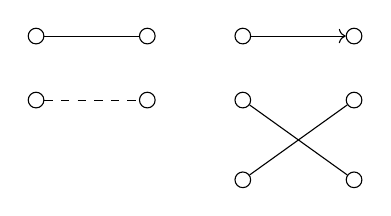
\begin{tikzpicture}[node distance=1.2cm, every node/.style={draw, circle, inner sep=2pt}]
    \node (A) {}; \node (B) [right=of A] {};
    \draw (A) -- (B);
    \node (C) [right=1cm of B] {}; \node (D) [right=of C] {};
    \draw [->] (C) -- (D);
    \node (E) [below=0.6cm of A] {}; \node (F) [right=of E] {};
    \draw [dashed] (E) -- (F);
    \node (G) [right=1cm of F] {}; \node (H) [right=of G] {};
    \node (I) [below=0.8cm of G] {}; \node (J) [below=0.8cm of H] {};
    \draw (G) -- (J);
    \draw (I) -- (H);
\end{tikzpicture}
\caption{Edge notation. Top left: two-way corridor. Top right: one-way
passage. Bottom left: labeled map-segment transition (stair), drawn dashed.
Bottom right: through passage --- movement only along the marked diagonals,
which do not connect where they cross.}
\label{fig:notation}
\end{figure}

\section{Routes: identity, shortest paths, enumeration}
\label{sec:routes}

\subsection{Route identity}

Enumerating all simple paths between two controls is exponential and mostly
meaningless: two paths that wiggle through different corridors of the same
floor are easily identified, and for orienteering purposes we can consider them the \emph{same route}. We therefore
define:

\begin{quote}
Two paths from control $A$ to control $B$ are the same \textbf{route} if and
only if they cross the same labeled edges (stairs) in the same order.
\end{quote}

The identity of a route is its \emph{label sequence} --- precisely the stair
notation of Section~\ref{sec:terminology}. The enumeration problem becomes:
find all distinct label sequences from $A$ to $B$, and for each, the shortest
concrete path realizing it.

\subsection{Cluster condensation}

Bidirectional unlabeled edges never contribute to route
identity: within a flat region, one can always take the cheapest corridor
path. The analysis therefore collapses every connected component of the
bidirectional-unlabeled subgraph into a single \emph{cluster} (using a
disjoint-set structure). One-way unlabeled edges are excluded from the merge
--- collapsing them would erase their directionality --- and instead become
directed edges of the condensed graph.

The resulting \textbf{cluster graph} has one node per connected region and one
directed edge per traversable direction of each stair or one-way passage
(Figure~\ref{fig:clusters}). Each physical staircase may be used at most once
per route (in either direction); this single constraint bounds the search
space while still allowing a route to revisit the same floor via
different stairs --- a real phenomenon in multi-floor venues.

\begin{figure}[h]
\centering
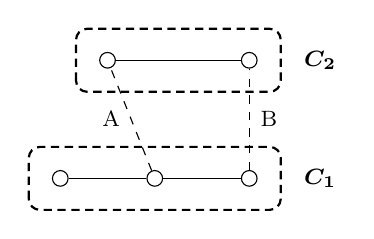
\begin{tikzpicture}[every node/.style={draw, circle, inner sep=2pt}]
    % Floor 1 corridor
    \node (n1) at (0,0) {};
    \node (n2) at (1.2,0) {};
    \node (n3) at (2.4,0) {};
    \draw (n1) -- (n2) -- (n3);
    % Floor 2 corridor
    \node (n4) at (0.6,1.5) {};
    \node (n5) at (2.4,1.5) {};
    \draw (n4) -- (n5);
    % Stairs
    \draw [dashed] (n2) -- (n4) node [draw=none, midway, left] {\footnotesize A};
    \draw [dashed] (n3) -- (n5) node [draw=none, midway, right] {\footnotesize B};
    % Cluster outlines: black, thick, dashed so they remain legible in
    % black-and-white printing.
    \draw [black, thick, dash pattern=on 3pt off 2pt, rounded corners]
        (-0.4,-0.4) rectangle (2.8,0.4);
    \draw [black, thick, dash pattern=on 3pt off 2pt, rounded corners]
        (0.2,1.1) rectangle (2.8,1.9);
    \node [draw=none] at (3.3,0) {\footnotesize $\boldsymbol{C_1}$};
    \node [draw=none] at (3.3,1.5) {\footnotesize $\boldsymbol{C_2}$};
\end{tikzpicture}\\[3pt]
\footnotesize (a) venue graph
\\[10pt]
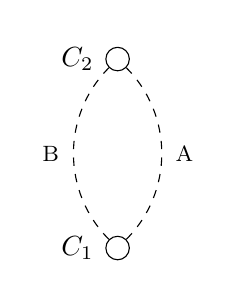
\begin{tikzpicture}[every node/.style={draw, circle, inner sep=3pt}]
    \node (C1) at (0,0)   {};
    \node (C2) at (0,2.4) {};
    \node [draw=none, left=3pt] at (C1) {$C_1$};
    \node [draw=none, left=3pt] at (C2) {$C_2$};
    \draw [dashed, bend left=45] (C1) to (C2);
    \draw [dashed, bend right=45] (C1) to (C2);
    \node [draw=none] at (0.85,1.2)  {\footnotesize A};
    \node [draw=none] at (-0.85,1.2) {\footnotesize B};
\end{tikzpicture}\\[3pt]
\footnotesize (b) condensed cluster graph
\caption{Cluster condensation. The corridors of each floor collapse into
clusters $C_1$ and $C_2$; the condensed graph (b) has exactly two edges,
stairs A and B. There are two distinct routes $C_1 \to C_2$: label sequences
$[A]$ and $[B]$, regardless of which corridors are walked.}
\label{fig:clusters}
\end{figure}

\subsection{Algorithms}

Four algorithm families operate on this model; full derivations and
implementation notes are given in the repository's algorithm
reference~\cite{repo}.

\textbf{Shortest path.} Dijkstra's algorithm over the venue graph, with
edge weights as defined above. 

\textbf{Heuristic alternatives.} A $k$-shortest-paths heuristic in the family
of penalty methods: edges on previously found paths are made progressively
more expensive (level-change edges $\times 5.0$ per iteration, corridors
$\times 1.2$) and Dijkstra is re-run, diversifying stair choice aggressively.
Fast, but with no completeness guarantee.

\textbf{Exhaustive enumeration.} A best-first search over the cluster graph
enumerates \emph{all} distinct label sequences, shortest first. An exact,
admissible heuristic --- one Dijkstra run on the reversed full graph from the
target --- makes the search pop states in non-decreasing order of true route
length, so the first completion found for a given label sequence is its
shortest realization, and deduplication is a constant-time set lookup. Depth,
result-count, and distance-ratio guards keep the (theoretically exponential)
search practical; real venues have on the order of 10--20 stair edges and
produce route inventories in the hundreds.

\textbf{Human-route simulation.} A fourth algorithm deliberately does not
seek the optimal route: it simulates the bounded, satisficing search a human
competitor performs under map-reading and working-memory constraints, on the
same cluster graph. It short-circuits legs solvable within a single cluster,
otherwise runs an alternating bidirectional search that expands the
nearest, goal-directed stair on each side in turn and stops at the first
meeting point, without backtracking to consider alternatives. The result is
a single, non-optimal, deterministic route that can be compared against the
enumerated optimum, giving measures --- such as the human--optimal length gap
--- that a purely optimal analysis cannot provide. This algorithm and its
cognitive motivation are developed in a companion
article~\cite{human-route}.

\section{Difficulty scoring}
\label{sec:scoring}

\subsection{Architecture}

Difficulty scoring is isolated behind a pluggable \emph{scoring model}
interface: a model receives the graph, and a concrete route, and returns a score. This separation is deliberate ---
the framework is designed to host competing models so they can be compared
against the same route inventories and empirical data.

\subsection{The difficulty model}

The first model is intentionally simple: a linear combination of two
structural counts,

\[
D \;=\; k \bigl(5\,N_f + 3\,N_b\bigr), \qquad k = \frac{100}{81}
\]

where, for the scored route,

\begin{itemize}
    \item $N_f$ is the number of stair (floor-change) traversals, upward and
          downward combined (an edge counts as a stair when its endpoints
          resolve to different floor levels);
    \item $N_b$ is the number of \emph{branching points}: route nodes at
          which more than one next node is reachable (excluding the node
          just come from, and respecting one-way constraints);
    \item $k = 100/81$ is a scaling factor that normalizes a reference leg
          (Stockholm Indoor Cup 2023, stage 1, course 1, leg 3$\to$4; raw
          score 81) to exactly 100.
\end{itemize}

The term weights, 5 for a stair crossing and 3 for a branching point, were
assigned arbitrarily, by judgment rather than by fitting to empirical data;
only the scaling factor $k$ is calibrated, and only against a single
reference leg. Establishing whether these particular weights are justified
is exactly the empirical validation work described in
Section~\ref{sec:research}.

Leg difficulty is the difficulty score of the leg's shortest route; course
difficulty defaults to the \emph{maximum} leg difficulty (a course is as hard
as its hardest leg), with the mean reported as a secondary statistic. Scores
map onto the five-color scale at fixed thresholds
(Table~\ref{tab:thresholds}).

\begin{table}[h]
\centering
\begin{tabular}{@{}ll@{}}
\toprule
\textbf{Category} & \textbf{Score range} \\ \midrule
White  & $0$--$20$  \\
Yellow & $20$--$40$ \\
Orange & $40$--$60$ \\
Purple & $60$--$80$ \\
Black  & $80+$      \\ \bottomrule
\end{tabular}
\caption{Difficulty scores mapped to difficulty categories.}
\label{tab:thresholds}
\end{table}

\subsection{Refinements}

Raw branching counts every fork, including trivially dismissible ones. Two
refinements are computed alongside the score and available to future models:

\begin{itemize}
    \item \textbf{Dead-end filtering:} edges on non-branching chains that
          terminate at a leaf are excluded --- a passage with only one way in
          and out creates no real decision.
    \item \textbf{Decision points:} a stricter variant that counts a node
          only when an off-route branch is \emph{significant}, i.e.\ runs at
          least 50 m before dead-ending or rejoining the route. A 10 m alcove
          is visibly wrong and creates no decision; a 50 m parallel corridor
          is a genuine route choice.
\end{itemize}

\subsection{Known limitations}

This model is a baseline, and its limitations chart the research agenda:
branching is counted, not weighted by how hard the
alternatives are to reject; the additive form cannot express the
combinatorial explosion of several \emph{sequential} decisions; and the score
depends on how densely the navigation graph is drawn, so graph-drawing
conventions must be standardized before scores are comparable across venues.

\section{Implementation and data}
\label{sec:implementation}

The framework is implemented as an open-source toolchain~\cite{repo}: a
client-side web application for drawing venue graphs over competition maps,
setting courses, and inspecting route inventories and difficulty scores; and
command-line tools for batch analysis, format conversion (JSON, IOF XML 3.0,
CSV, GPX), and video visualization of the route-finding algorithms. Venue
graphs, courses, and analysis results use documented schemas so that datasets
are portable.

The repository also contains anonymized split-time data from real indoor
events (per-leg times from public results services), joined with computed
per-leg difficulty scores. This dataset is the basis for the validation work
described next; no validation results are claimed in this article.

\section{Research directions}
\label{sec:research}

The framework is a foundation. Directions we consider promising, roughly in
order of dependency:

\begin{enumerate}
    \item \textbf{Empirical validation.} Correlate per-leg difficulty scores
          with observed performance (time loss relative to the leg winner,
          spread of split times, and mistake frequency) across the
          collected event data, per difficulty category and runner class.
    \item \textbf{Model competition.} Fit alternative scoring models (e.g.\
          weighting decision points by branch significance, multiplicative or
          entropy-based forms) against the same data, using the pluggable
          model interface, and compare predictive power.
    \item \textbf{Route-choice entropy.} The exhaustive route inventory
          enables information-theoretic measures: a leg where several routes
          have near-equal length carries more decision load than one with a
          single dominant route. Quantify this and test it as a model term.
    \item \textbf{Trap detection.} Compare the geometrically shortest route
          with the lowest-difficulty route; large divergence signals
          course-setter ``baits'' worth flagging automatically.
    \item \textbf{Human route modeling.} Predict which of the enumerated
          routes runners actually take, and how the choice depends on experience level.
    \item \textbf{Graph-drawing norms.} Establish conventions for node and
          edge placement density so difficulty scores are comparable across
          venues and mappers.
    \item \textbf{Training effects.} Study whether targeted practice 
          shifts the difficulty--performance relationship.
\end{enumerate}

\section{Conclusion}

We have introduced a graph-based framework for indoor orienteering course
analysis: a venue model capturing stairs, one-way constraints, and floor
membership; a definition of route identity via stair-label sequences that
makes exhaustive route enumeration tractable; and a first, deliberately
simple difficulty scoring model aligned with the established difficulty
categories. All components are implemented in an open toolchain. 
The intended contribution is a foundation:
a shared vocabulary and testable baseline against which better models of
indoor navigational difficulty can now be built.

\begin{thebibliography}{9}

\bibitem{norm-indoor}
Indoor-projektet (2023). \emph{Norm f\"or banl\"aggning inom Indoor i
Sverige}.

\bibitem{wettergren2024}
Johan Wettergren (2024). \emph{R\r{a}d till banl\"aggare av
inomhusorientering}.

\bibitem{sic-difficulty}
Stockholm Indoor Cup. \emph{Sv\r{a}righetsgrader --- Difficulty levels}.

\bibitem{repo}
\emph{Indoor Orienteering Route Analysis} (source code, algorithm reference,
and datasets). \newblock
\url{github:objorke/indoor-o-route-analysis}.

\bibitem{human-route}
\emph{How humans solve indoor orienteering courses}. Companion article, same
repository.

\end{thebibliography}

\end{document}
